\section{Scoring}

\subsection{Key Signatures}
\todo[inline,color=red]{Scoring Techniques - Key Signatures}

\subsection{Beats and Timing}
\todo[inline,color=red]{Scoring Techniques - Beats and Timing}

\subsection{Stems}

\subsubsection{Stem Angle}
\todo[inline,color=red]{Scoring Techniques - Stem Angle}
 \begin{figure}[h!]
        \centering
        \tiny
        \addtolength{\subfigcapskip}{0.2cm}

        \subfigure[-23.9]{
          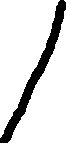
\includegraphics[height=2cm,keepaspectratio]{gfx/implementation/stem-angle/4883.png}
          \label{fig:stem-angle-4883}
        }
        \quad
        \subfigure[-20.0]{
          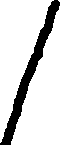
\includegraphics[height=2cm,keepaspectratio]{gfx/implementation/stem-angle/4718.png}
          \label{fig:stem-angle-4718}
        }
        \quad
        \subfigure[18.7]{
          
\includegraphics[height=2cm,keepaspectratio]{gfx/implementation/stem-angle/4705.png}
          \label{fig:stem-angle-4705}
        }
        \quad
        \subfigure[-14.7]{
          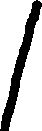
\includegraphics[height=2cm,keepaspectratio]{gfx/implementation/stem-angle/4886.png}
          \label{fig:stem-angle-4886}
        }
        \quad
        \subfigure[-9.8]{
          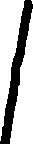
\includegraphics[height=2cm,keepaspectratio]{gfx/implementation/stem-angle/4892.png}
          \label{fig:stem-angle-4892}
        }
        \quad
        \subfigure[-8.4]{
          
\includegraphics[height=2cm,keepaspectratio]{gfx/implementation/stem-angle/4645.png}
          \label{fig:stem-angle-4645}
        }
        \quad
        \subfigure[7.3]{
          
\includegraphics[height=2cm,keepaspectratio]{gfx/implementation/stem-angle/3889.png}
          \label{fig:stem-angle-3889}
        }
        \quad
        \subfigure[6.2]{
          
\includegraphics[height=2cm,keepaspectratio]{gfx/implementation/stem-angle/5380.png}
          \label{fig:stem-angle-5380}
        }
        \quad
        \subfigure[5.1]{
          
\includegraphics[height=2cm,keepaspectratio]{gfx/implementation/stem-angle/4194.png}
          \label{fig:stem-angle-4194}
        }
        \quad
        \subfigure[-4.1]{
          
\includegraphics[height=2cm,keepaspectratio]{gfx/implementation/stem-angle/3970.png}
          \label{fig:stem-angle-3970}
        }
        \quad
        \subfigure[3.0]{
          
\includegraphics[height=2cm,keepaspectratio]{gfx/implementation/stem-angle/4783.png}
          \label{fig:stem-angle-4783}
        }
        \quad
        \subfigure[2.0]{
          
\includegraphics[height=2cm,keepaspectratio]{gfx/implementation/stem-angle/3920.png}
          \label{fig:stem-angle-3920}
        }
        \quad
        \subfigure[-1.0]{
          
\includegraphics[height=2cm,keepaspectratio]{gfx/implementation/stem-angle/5368.png}
          \label{fig:stem-angle-5368}
        }
        \quad

        \caption{Ranking of stems according to their off-vertical angle}
        \label{fig:stem-angle-ranking}
      \end{figure}



\subsubsection{Stem Straightness}

Given a drawn note stem, we wish to be able to determine a measure of `straightness' which we can threshold to discern a badly drawn stem shown in \cref{fig:wonky-stems} from a straight one  as shown in \cref{fig:straight-stems}.

\begin{figure}[h!]
    \centering
    \begin{subfigure}[b]{.4\linewidth}
        \centering
        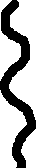
\includegraphics[height=4cm]{gfx/implementation/stem-straightness/4912.png}
        \quad
        
\includegraphics[height=4cm]{gfx/implementation/stem-straightness/5371.png}
        \caption{Examples of uneven stems}
        \label{fig:wonky-stems}
    \end{subfigure}
    \begin{subfigure}[b]{.4\linewidth}
        \centering
        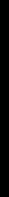
\includegraphics[height=4cm]{gfx/implementation/stem-straightness/3876.png}
        \quad
        
\includegraphics[height=4cm]{gfx/implementation/stem-straightness/5104.png}
        \caption{Examples of straight stems}
        \label{fig:straight-stems}
    \end{subfigure}

    \caption{Examples of straight and uneven stems}
    \label{fig:stem-straightness-examples}
\end{figure}

Stem straightness is different to the stem angle because intuitively even if the stem is angled, it can still be straight. Therefore, we need to establish a technique which gives a measure irrespective of them stem angle.

To do this, we take the original stem (\cref{fig:straight-skeleton-original}) and generate it's skeletal representation using techniques outlined in \cref{sec:skeletonization} which approximates a line following the center of the stem (\cref{fig:straight-skeleton-skeleton}). If we treat this skeleton as a plot of points, we can draw a line of best fit through them to approximate what a perfectly straight version of the stem (\cref{fig:straight-skeleton-bestfit}).

\begin{figure}[h!]
    \centering

    \begin{subfigure}[b]{.3\linewidth}
        \centering
        \frame{
\includegraphics[height=3cm]{gfx/techniques/skeletonization/4705.png}}
        \frame{
\includegraphics[height=3cm]{gfx/techniques/skeletonization/4912.png}}
        \caption{Original}
        \label{fig:straight-skeleton-original}
    \end{subfigure}
    \begin{subfigure}[b]{.3\linewidth}
        \centering
        \frame{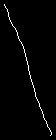
\includegraphics[height=3cm]{gfx/techniques/skeletonization/4705_skeleton.png}}
        \frame{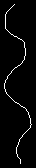
\includegraphics[height=3cm]{gfx/techniques/skeletonization/4912_skeleton.png}}
        \caption{Skeleton}
        \label{fig:straight-skeleton-skeleton}
    \end{subfigure}
    \begin{subfigure}[b]{.3\linewidth}
        \centering
        \frame{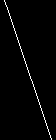
\includegraphics[height=3cm]{gfx/techniques/skeletonization/4705_bestfit.png}}
        \frame{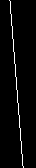
\includegraphics[height=3cm]{gfx/techniques/skeletonization/4912_bestfit.png}}
        \caption{Best Fit}
        \label{fig:straight-skeleton-bestfit}
    \end{subfigure}

    \caption{Examples of stem skeletons}
    \label{fig:stem-skeletons}
\end{figure}

We now have a skeleton line \cref{eqn:l-skeleton} and a best fit line \cref{eqn:l-ref} we can calculate the difference at each point \cref{eqn:l-residuals}.

\begin{equation} \label{eqn:l-skeleton}
    L_{\text{skeleton}}(x) = (a_0, a_1, a_2, \ldots, a_n)
\end{equation}
\begin{equation} \label{eqn:l-ref}
    L_{\text{ref}}(x) = (b_0, b_1, b_2, \ldots, b_n)
\end{equation}
\begin{equation} \label{eqn:l-residuals}
    R(x) = (r_0, r_1, r_2, \ldots, r_n), r_i = a_i - b_i)
\end{equation}


After experimenting with using the standard deviation \cref{eqn:sd} of the residuals as the straightness measure the results turned out to be positive upon visual inspection. As you can see in \cref{fig:stem-straightness-ranking} when ranked according to their `straightness' measure, the stems do indeed appear to be ordered according to what one would visually define as being `straight'.

\begin{equation} \label{eqn:sd}
\sigma = \sqrt{\frac{\sum\limits_{i=1}^{n}\left(r_{i} - \bar{r}\right)^{2}}{n-1}}
\end{equation}


\begin{figure}[h!]
  \centering
  \tiny
  \captionsetup[subfigure]{labelformat=empty}

  \subcaptionbox{7.3\label{fig:stem-straightness-4912}}[0.04\linewidth]{
    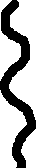
\includegraphics[height=1.5cm,keepaspectratio]{gfx/implementation/stem-straightness/4912.png}
  }
  \subcaptionbox{3.3\label{fig:stem-straightness-3889}}[0.04\linewidth]{
    
\includegraphics[height=1.5cm,keepaspectratio]{gfx/implementation/stem-straightness/3889.png}
  }
  \subcaptionbox{3.1\label{fig:stem-straightness-4064}}[0.04\linewidth]{
    
\includegraphics[height=1.5cm,keepaspectratio]{gfx/implementation/stem-straightness/4064.png}
  }
  \subcaptionbox{2.7\label{fig:stem-straightness-5371}}[0.04\linewidth]{
    
\includegraphics[height=1.5cm,keepaspectratio]{gfx/implementation/stem-straightness/5371.png}
  }
  \subcaptionbox{2.5\label{fig:stem-straightness-3796}}[0.04\linewidth]{
    
\includegraphics[height=1.5cm,keepaspectratio]{gfx/implementation/stem-straightness/3796.png}
  }
  \subcaptionbox{2.4\label{fig:stem-straightness-3845}}[0.04\linewidth]{
    
\includegraphics[height=1.5cm,keepaspectratio]{gfx/implementation/stem-straightness/3845.png}
  }
  \subcaptionbox{2.2\label{fig:stem-straightness-4055}}[0.04\linewidth]{
    
\includegraphics[height=1.5cm,keepaspectratio]{gfx/implementation/stem-straightness/4055.png}
  }
  \subcaptionbox{1.8\label{fig:stem-straightness-4072}}[0.04\linewidth]{
    
\includegraphics[height=1.5cm,keepaspectratio]{gfx/implementation/stem-straightness/4072.png}
  }
  \subcaptionbox{1.6\label{fig:stem-straightness-4758}}[0.04\linewidth]{
    
\includegraphics[height=1.5cm,keepaspectratio]{gfx/implementation/stem-straightness/4758.png}
  }
  \subcaptionbox{1.5\label{fig:stem-straightness-4653}}[0.04\linewidth]{
    
\includegraphics[height=1.5cm,keepaspectratio]{gfx/implementation/stem-straightness/4653.png}
  }
  \subcaptionbox{1.4\label{fig:stem-straightness-4183}}[0.04\linewidth]{
    
\includegraphics[height=1.5cm,keepaspectratio]{gfx/implementation/stem-straightness/4183.png}
  }
  \subcaptionbox{1.2\label{fig:stem-straightness-4250}}[0.04\linewidth]{
    
\includegraphics[height=1.5cm,keepaspectratio]{gfx/implementation/stem-straightness/4250.png}
  }
  \subcaptionbox{1.1\label{fig:stem-straightness-4003}}[0.04\linewidth]{
    
\includegraphics[height=1.5cm,keepaspectratio]{gfx/implementation/stem-straightness/4003.png}
  }
  \subcaptionbox{0.9\label{fig:stem-straightness-5350}}[0.04\linewidth]{
    
\includegraphics[height=1.5cm,keepaspectratio]{gfx/implementation/stem-straightness/5350.png}
  }
  \subcaptionbox{0.8\label{fig:stem-straightness-4103}}[0.04\linewidth]{
    
\includegraphics[height=1.5cm,keepaspectratio]{gfx/implementation/stem-straightness/4103.png}
  }
  \subcaptionbox{0.7\label{fig:stem-straightness-5104}}[0.04\linewidth]{
    
\includegraphics[height=1.5cm,keepaspectratio]{gfx/implementation/stem-straightness/5104.png}
  }
  \subcaptionbox{0.6\label{fig:stem-straightness-4038}}[0.04\linewidth]{
    
\includegraphics[height=1.5cm,keepaspectratio]{gfx/implementation/stem-straightness/4038.png}
  }
  \subcaptionbox{0.5\label{fig:stem-straightness-4565}}[0.04\linewidth]{
    
\includegraphics[height=1.5cm,keepaspectratio]{gfx/implementation/stem-straightness/4565.png}
  }
  \subcaptionbox{0.4\label{fig:stem-straightness-4011}}[0.04\linewidth]{
    
\includegraphics[height=1.5cm,keepaspectratio]{gfx/implementation/stem-straightness/4011.png}
  }
  \subcaptionbox{0.3\label{fig:stem-straightness-3327}}[0.04\linewidth]{
    
\includegraphics[height=1.5cm,keepaspectratio]{gfx/implementation/stem-straightness/3327.png}
  }
  \subcaptionbox{0.2\label{fig:stem-straightness-4752}}[0.04\linewidth]{
    
\includegraphics[height=1.5cm,keepaspectratio]{gfx/implementation/stem-straightness/4752.png}
  }
  \subcaptionbox{0.1\label{fig:stem-straightness-3876}}[0.04\linewidth]{
    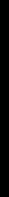
\includegraphics[height=1.5cm,keepaspectratio]{gfx/implementation/stem-straightness/3876.png}
  }
  \caption{Ranking of stems according to their `straightness' score}
  \label{fig:stem-straightness-ranking}
\end{figure}


\subsubsection{Stem Direction}

To establish the stem direction which I will refer to as $S_d$, the vertical position (y coordinates) of the head and the stem are compared.

If the stem is located at $(x_{\text{stem}}, y_{\text{stem}})$ and the note head at $(x_{\text{head}}, y_{\text{head}})$, knowing that the coordinate axes have an origin starting from the top right of a given image, we can establish the following classifications:

$$
S_{d} (y_{\text{stem}}, y_{\text{head}}) =
\left\{
	\begin{array}{ll}
		\text{up}   & \mbox{if } y_{\text{stem}} < y_{\text{head}} \\
		\text{down} & \mbox{if } y_{\text{stem}} > y_{\text{head}}
	\end{array}
\right.
$$

The case where a stem has the same $y$ coordinate as it's head isn't possible due to the way stems are extracted from a note complex as for this to happen a stem would need to be extracted \emph{out} of a note head. Since note heads are removed in order to identify stems as in \todo[color=blue]{REFERENCE: Extracting Stems}, this is impossible.

\begin{table}[h]

    \begin{tabularx}{\textwidth}{ X l l l l }
    \toprule
    Component & Stem Y   & Head Y   & Predicted Direction & True Direction \\
    \midrule
    \bottomrule
    \end{tabularx}

    \label{table:stem-direction-results}
    \caption{Results of the stem direction classification heuristic}
\end{table}
\todo[inline,color=purple]{Stem Direction: Results Table (Showing stems and classification of up/down)}



\subsubsection{Stem Side}
To establish the stem side which I will refer to as $S_s$, we do a similar operation to in determining the direction, however, since it is perfectly feasible that the stem and head have the same x coordinate, we can't just use the x coordinate directly.

Instead, we compare the x coordinate of the stem $x_{\text{stem}}$ to the true centre \todo{Better definition later please} of the note head $cx_{\text{head}}$

Again, given that the coordinate axes start from the top left, we can now establish the stem x offset

$$
S_\text{xoff} = x_{\text{stem}} - cx_{\text{head}}
$$

Using this, we can establish the side classification as
$$
S_{s} (S_\text{xoff}) =
\left\{
	\begin{array}{ll}
		\text{left}   & \mbox{if } S_\text{xoff} < 0 \\
		\text{right}  & \mbox{if } S_\text{xoff} \ge 0
	\end{array}
\right.
$$

\subsubsection{Stem Length}

Stem length may seem like a simple case of measuring the length of the extracted stem, but it's actually a little more complicated. In order to get the best results, we need to take into account the fact that the stem has been extracted from the note head and that this separation point could occur anywhere from near the bottom as in \cref{fig:stem-separation-bottom} to the top as in \cref{fig:stem-separation-top}.

\begin{figure}[h!]
    \centering

    \begin{subfigure}[b]{.3\linewidth}
        \centering
        \missingfigure{Stem coming out the top of a note head}
        \caption{Original}
        \label{fig:stem-separation-top}
    \end{subfigure}
    \begin{subfigure}[b]{.3\linewidth}
        \centering
        \missingfigure{Stem coming out the bottom of a note head}
        \caption{Best Fit}
        \label{fig:stem-separation-bottom}
    \end{subfigure}

    \caption{Examples of stem and note head intersection points}
\end{figure}

Similarly to the straightness and angular measures, we can establish the raw length $L_R$ by drawing a line through the perceived centre of the stem and measuring it's length using simple trigonometry. However, although it might seem counterintuitive to not use this as a measure of length, in reality a better measure of whether the stem is `too long' is to measure the distance between the stave line/space above stem's associated notehead and the y coordinate of the stem.

If we define the correct length $L_E$ for a stem as outlined in \todo{REFERENCE where I talk about correct stem length} then the length score is therefore just $L_E - L_A$ where smaller values mean the stem is closer to the expected length.

\subsection{Quaver Tail Side}
\todo[inline,color=red]{Scoring Techniques - Quaver tail side}

\subsection{Note Heads}
\todo[inline,color=red]{Scoring Techniques - Note Head - Filled Percentage?? (ambiguity)}
\todo[inline,color=red]{Scoring Techniques - Note Head - Gaps/broken circles}
\todo[inline,color=red]{Scoring Techniques - Note Head - Eccentricity?}
